\documentclass[a4paper,
fontsize=11pt,
%headings=small,
oneside,
numbers=noperiodatend,
parskip=half-,
bibliography=totoc,
final
]{scrartcl}

\usepackage{synttree}
\usepackage{graphicx}
\setkeys{Gin}{width=.6\textwidth} %default pics size

\graphicspath{{./plots/}}
\usepackage[ngerman]{babel}
%\usepackage{amsmath}
\usepackage[utf8x]{inputenc}
\usepackage [hyphens]{url}

\usepackage[colorlinks, linkcolor=black,citecolor=black, urlcolor=blue,
breaklinks= true]{hyperref}
\usepackage{booktabs} 
\usepackage[left=2.4cm,right=2.4cm,top=2.3cm,bottom=2cm,includeheadfoot]{geometry}
\usepackage{eurosym}
\usepackage{multirow}
\usepackage[ngerman]{varioref}
\setcapindent{1em}
\renewcommand{\labelitemi}{--}
\usepackage{paralist}
\usepackage{pdfpages}
\usepackage{lscape}
\usepackage{float}
\usepackage{acronym}
\usepackage{eurosym}
\usepackage[babel]{csquotes}
\usepackage{longtable,lscape}
\usepackage{mathpazo}
\usepackage[flushmargin,ragged]{footmisc} % left align footnote

\urlstyle{same}  % don't use monospace font for urls

\usepackage[fleqn]{amsmath}

%adjust fontsize for part

\usepackage{sectsty}
\partfont{\large}

%Das BibTeX-Zeichen mit \BibTeX setzen:
\def\symbol#1{\char #1\relax}
\def\bsl{{\tt\symbol{'134}}}
\def\BibTeX{{\rm B\kern-.05em{\sc i\kern-.025em b}\kern-.08em
    T\kern-.1667em\lower.7ex\hbox{E}\kern-.125emX}}

\usepackage{fancyhdr}
\fancyhf{}

\pagestyle{fancyplain}

\fancyhead[R]{\thepage}
%meta

\fancyhead[L]{C. Haas \& B. Rusch \\ % author
LIBREAS. Library Ideas, 24 (2014) % journal, issue, volume
\href{http://nbn-resolving.de/urn:nbn:de:kobv:11-100215873}{urn:nbn:de:kobv:11-100215873}} %urn
\fancyfoot[L] {\textit{Creative Commons BY 3.0}} %licence
\fancyfoot[R] {\textit{ISSN: 1860-7950}}

\title{\LARGE{Piraten und Kapitalisten denken eine globale digitale Bibliothek. Eindrücke von der \enquote{Complicity – Berliner Gazette Konferenz 2013}}} %title
\author{Corinna Haas \& Beate Rusch} %author

\date{}

\begin{document}

\maketitle
\thispagestyle{fancyplain} 



\begin{center}
\sffamily{\textbf{ABSTRACT}}
\end{center}

\begin{abstract}
\small
Wie können \enquote{Piraten} und \enquote{Kapitalisten} zusammenarbeiten? Welche Komplizenschaften können Hacker und Journalisten, Profis und Amateure miteinander eingehen, wenn es darum geht, die Informationsfreiheit im Internet zu verteidigen? Diesen Fragen ging die \enquote{Complicity – Berliner Gazette Konferenz 2013} im Berliner SUPERMARKT nach. Die Autorinnen kommentieren die Konferenz aus ihrer Perspektive als Teilnehmerinnen. Ihr Beitrag reflektiert die Konfrontation von Bibliotheksutopie und Bibliotheksrealität, den \enquote{piratischen} Umgang mit Urheberrechtsproblemen und Open Access sowie die Interessenkonvergenzen von Bibliothekaren und Internetaktivisten
\end{abstract}

\begin{abstract}
\small
How can pirates and capitalists work together? And how is it possible for hackers and journalists, professionals and amateurs to enter into complicity, in order to defend the freedom of information on the web? These were the issues the \enquote{Complicity – Berliner Gazette Conference 2013} dealt with at the SUPERMARKT in Berlin. The authors comment on the conference from a participant’s point of view. Their contribution reflects confrontations of utopias and realities of the library, \enquote{pirate} ways to deal with copyright problems and Open Access, as well as the convergence of interests between librarians and internet activists.
\end{abstract}

\begin{center}\rule{3in}{0.4pt}\end{center}


\section*{Das Setting}\label{das-setting}

Wie können \enquote{Piraten und Kapitalisten} zusammenarbeiten? Fünfzehn
Menschen, die meisten zwischen 25 und 35 Jahre alt und im Auftreten eher
lässig als \emph{businesslike}, wollen es herausfinden. Die Gruppe
schart sich mit ihren Laptops um eine Mehrfachsteckdose wie um ein
Herdfeuer. Nicht weit entfernt davon versammeln sich \enquote{Hacker und
Journalisten} sowie \enquote{Profis und Amateure}, um mögliche
Verbindungen und Kooperationen zwischen ungleichen Partnern auszuloten.

Doch wer ist hier wer? Der Einladung des Veranstalters \enquote{Berliner
Gazette} sind etwa 50 Künstler, Journalisten, Hacker,
Kulturwissenschaftler, Soziologen, Juristen und auch zwei
Bibliothekarinnen gefolgt. Viele stammen aus Berlin und Deutschland.
Andere kommen aus Spanien, Portugal und Griechenland -- den
Krisenländern, Weißrussland und Mazedonien -- Ländern mit aktueller
Zensurerfahrung, sowie Kroatien, wo die Erinnerungen an Nationalismus
und Krieg noch frisch sind. Der Horizont ist also weit gespannt, die
Hintergründe sind vielfältig. Man spricht Englisch. Alle Anwesenden sind
aktiv, ein passives Publikum ist nicht vorgesehen.

\begin{figure}[htbp]
\centering
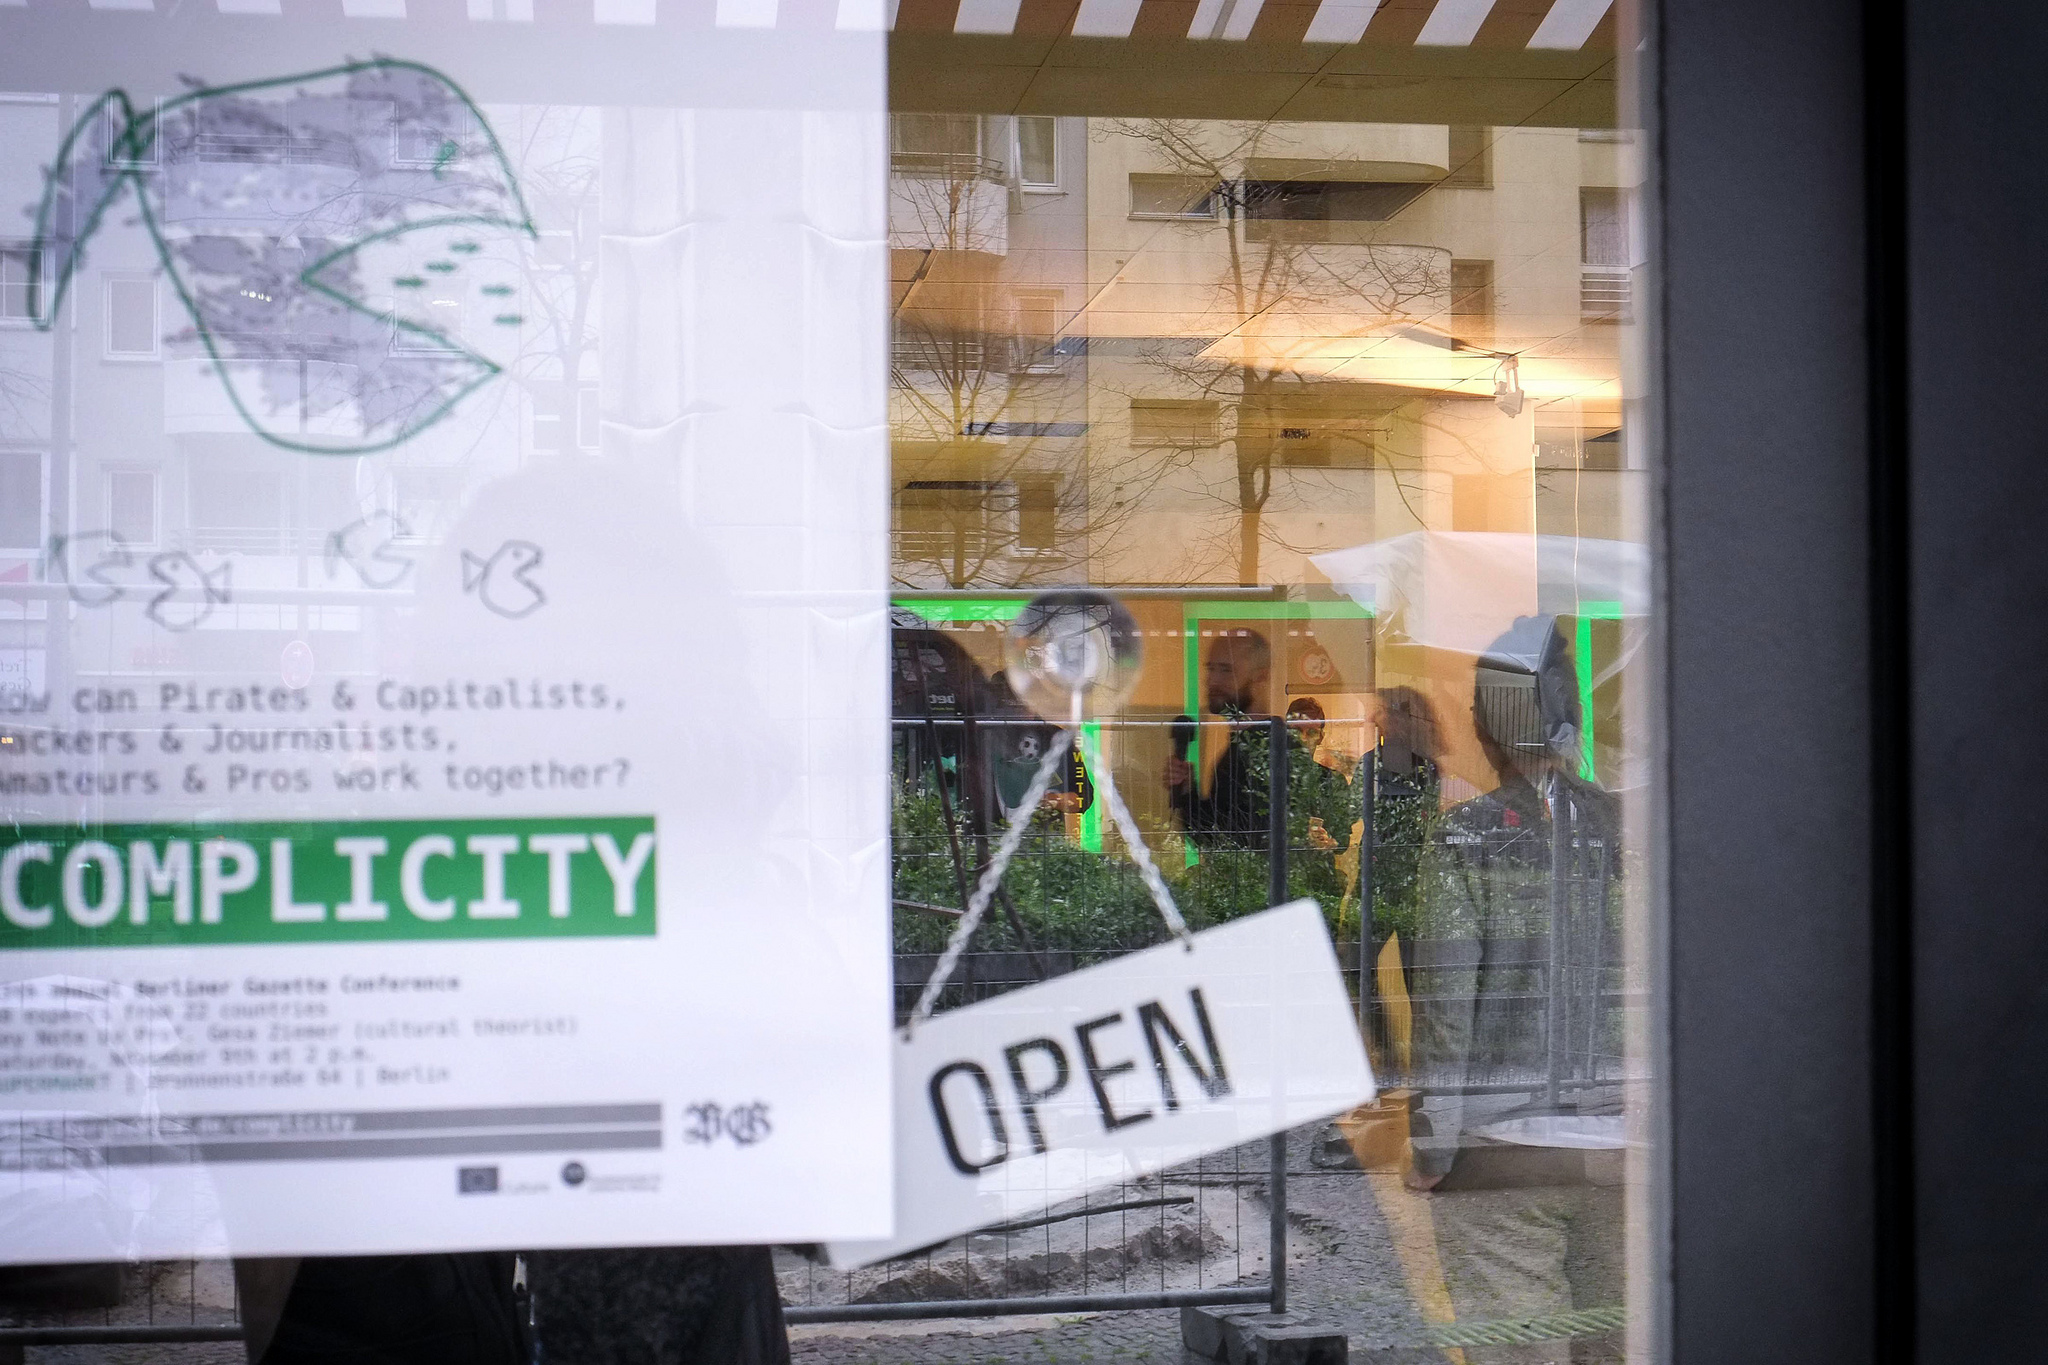
\includegraphics{./img/Konferenzposter.jpg}
\caption{Konferenzposter}
\end{figure}

Wir sind bei der 13. Jahreskonferenz der Berliner Gazette, eines
erfolgreichen Berliner Online-Magazins zu Journalismus, Kunst und
Wissenschaft.\footnote{Konferenzwebsite:
  \url{http://berlinergazette.de/symposium/complicity/}} Die Berliner
Gazette wurde 1999 von Krystian Woznicki als Feuilleton und
experimentelle Plattform im Internet gegründet. Woznicki,
Chefredakteurin Magdalena Taube und ihr Team verbinden
Online-Journalismus mit Offline-Aktivitäten: Sie organisieren Symposien
und Seminare zur Medienkultur und kooperieren dabei mit Partnern wie
Kulturinstitutionen, politischen Stiftungen, Schulen und Hochschulen.
Jedes Jahr wählt die Berliner Gazette ein Schwerpunktthema.\footnote{\url{http://berlinergazette.de/ueber-uns/}}
Die Complicity-Konferenz vom 7. bis 9. November 2013 bildet den Auftakt
für das Jahresthema 2014. Tagungsort ist der SUPERMARKT in
Berlin-Wedding.\footnote{\url{http://www.supermarkt-berlin.net/}}. Vor
wenigen Jahren ratterten in der schmucklosen Betonhalle noch
Einkaufswagen zwischen Regalen entlang. Nach der Schließung des
Discounters und einer Phase des Leerstandes gründeten Ela Kagel, David
Farine und Zsolt Szentirmai im Jahr 2010 den SUPERMARKT neu -- als
Konferenz- und Workshopzentrum, Café und Coworking Space. Wenn nicht
gerade die Berliner Gazette hier tagt, wird er von Berliner
Internetaktivisten und jungen Start-Ups genutzt.

Die Atmosphäre während der drei Konferenztage im November 2013 ist
entspannt und hoch konzentriert zugleich. Während morgens der geplante
Anfangszeitpunkt verstreicht, kommt man bei Kaffee und Croissants schon
einmal mit anderen Teilnehmern ins Gespräch. In den Workshops wird dann
so leidenschaftlich diskutiert, dass darüber die Pizza kalt wird; doch
unaufgeregte Moderatoren behalten die Lage unter Kontrolle. Und da hier
schon von \enquote{Konferenzkultur} die Rede ist: Eine gute
Gedächtnisstütze und zugleich ästhetisch reizvoll sind die \emph{Graphic
Recordings}, mit denen eine Do-It-Yourself-Masterklasse des SUPERMARKTs
(Leitung: Gabriele Schlipf, momik Berlin) die Workshops live
dokumentiert.

\section*{Die Aufgabe}\label{die-aufgabe}

Warum heißen wir eigentlich \enquote{Piraten und Kapitalisten}, und wer
ist wer? In der Vorstellungsrunde wird deutlich: Fassen wir unter
\enquote{Piraten} die Aktivisten, die für eine freie Grundstruktur des
Internet und für Informationsfreiheit eintreten, dann sind wir fast alle
Piraten. Allerdings distanzieren sich einige Teilnehmer entschieden von
Formen \enquote{piratischen} Handelns wie dem illegalen Filesharing in
Datenbanken - etwa der Musiker, der es ablehnt, \enquote{to rip off
someone else's stuff}. \enquote{Kapitalisten}, da ist sich die Gruppe
einig, sind die \emph{Global Players}wie Google und Amazon, die durch
ihre kommerziellen Interessen die Freiheit im Internet gefährden.
Vielleicht nicht überraschend, will sich unter uns kein Kapitalist
finden.

\begin{figure}[htbp]
\centering
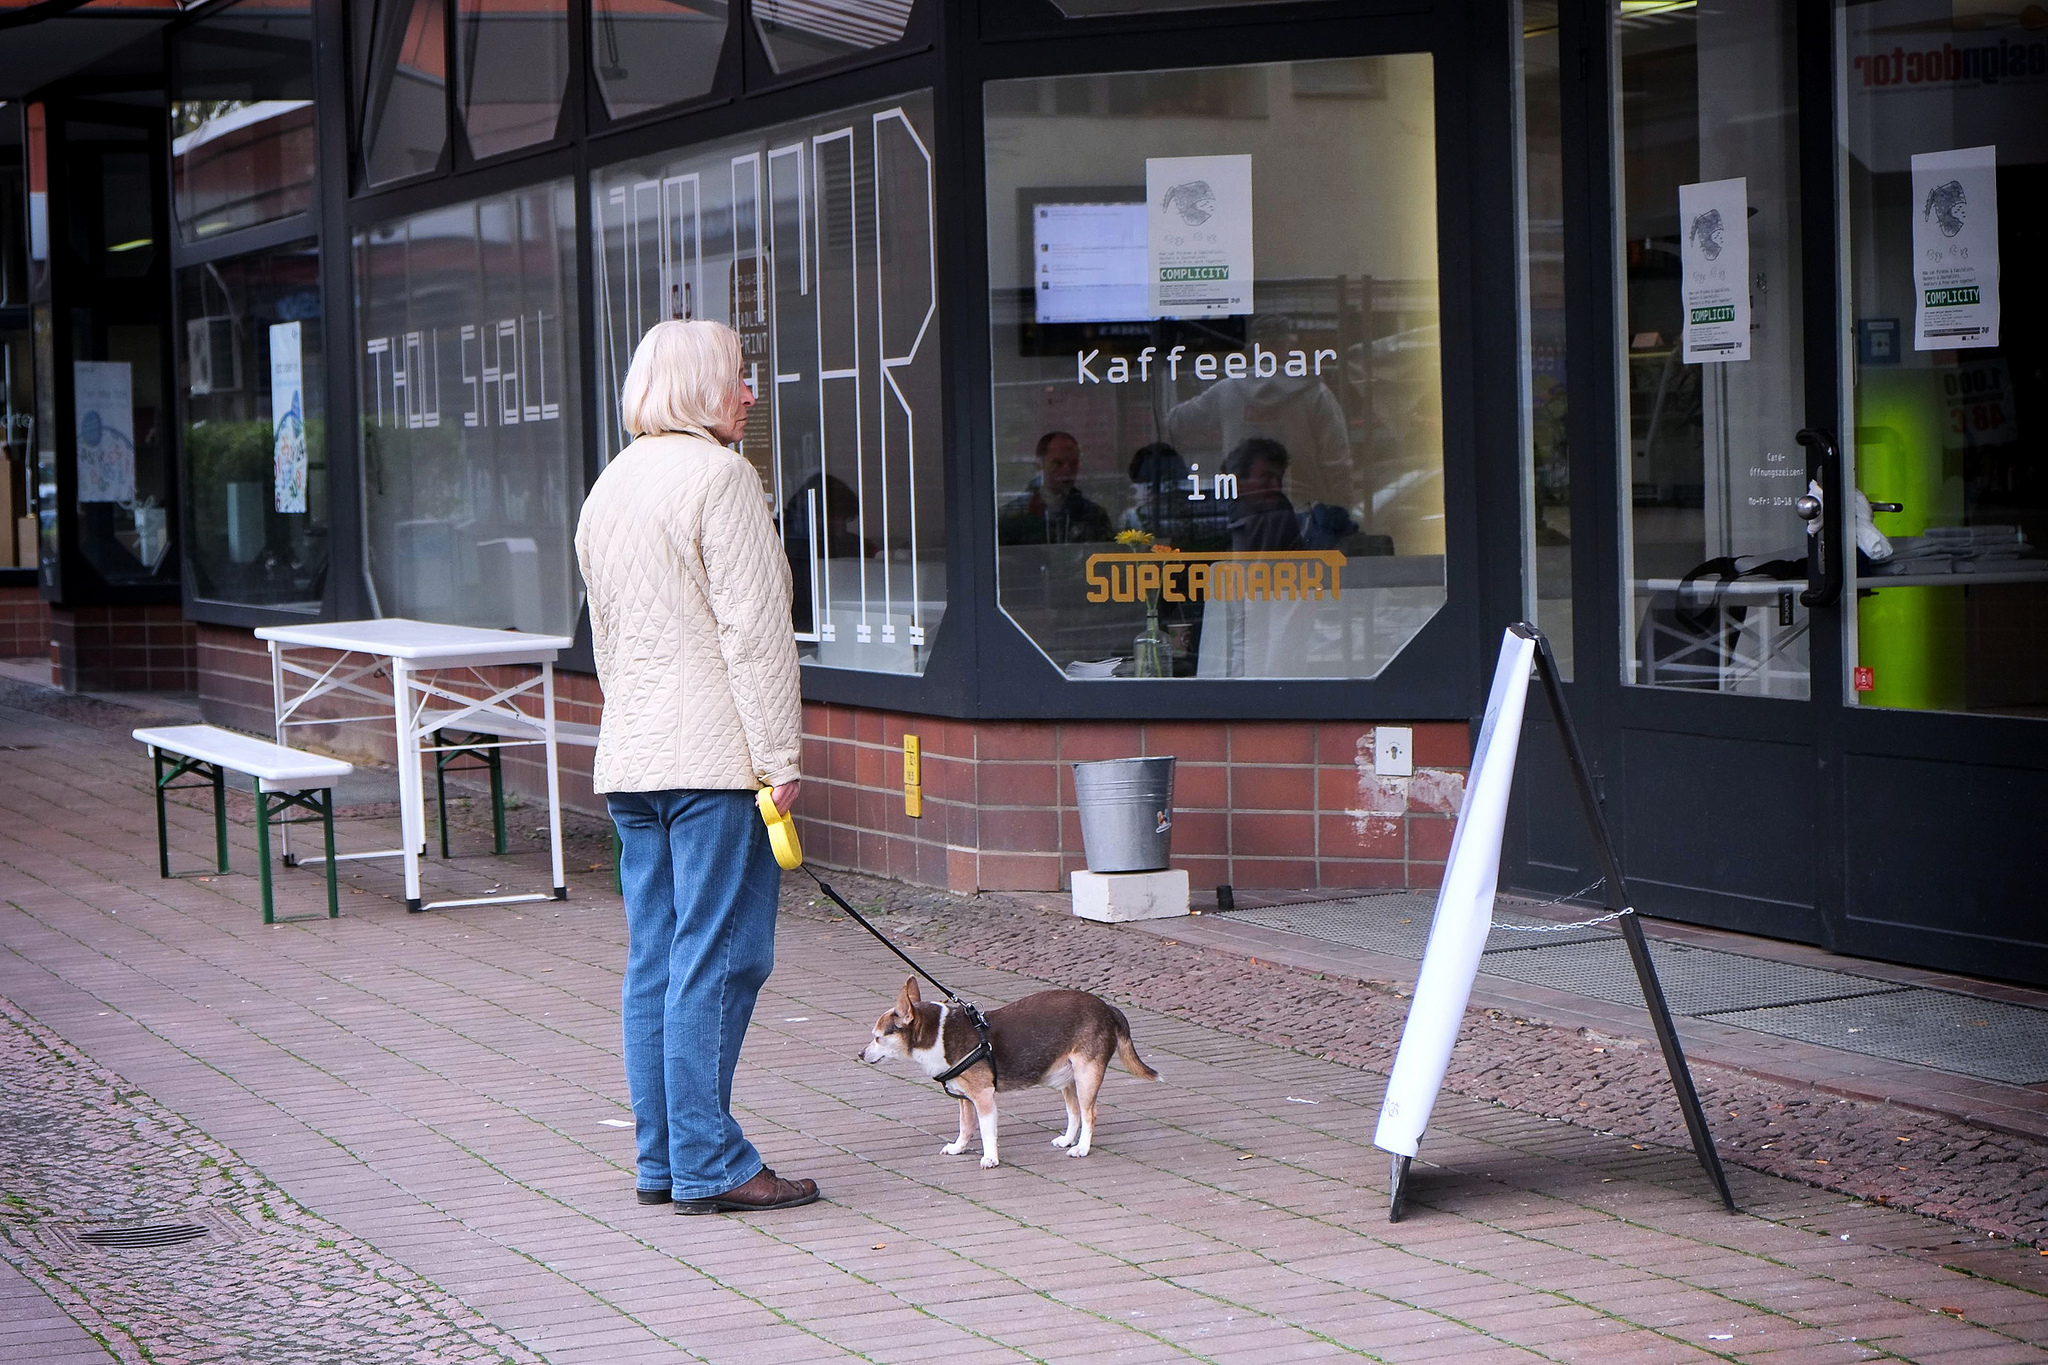
\includegraphics{./img/Supermarkt.jpg}
\caption{Supermarkt}
\end{figure}

Den Workshop moderieren der Hacker-Künstler Nenad Romić´ alias Marcell
Mars aus Zagreb und der Berliner Chris Piallat, Redaktionsmitglied der
Berliner Gazette sowie Referent für Netzpolitik bei den Grünen.

Marcell Mars' Eingangsreferat führt uns in das Szenario einer utopischen
virtuellen globalen Public Library mit Sitz in Island ein und setzt
Impulse für das Rollenspiel der Gruppe: \emph{Stellt euch vor, ein
ganzes Land agierte piratisch. Stellt euch vor, das kleine Land Island
spielte den Vorreiter und würde das gesamte Wissen digital verfügbar
machen und eine digitale Bibliothek aufbauen. Welche gesellschaftlichen,
kulturellen und wirtschaftlichen Folgen würden sich daraus ergeben?}
Dass die traditionelle Institution Bibliothek obsolet sei, setzt dieses
Szenario gleichsam voraus: Seit der Digitalisierung sei sie von
kommerziellen Interessen bedroht und durch das geltende Copyright
geknebelt. Auch könne sie die Ansprüche ihrer Klientel längst nicht mehr
erfüllen, die sich deshalb eigene, oft illegale Informationsstrukturen
aufbauten.~

Diese Idee einer globalen, digitalen Bibliothek setzt schnell
Assoziationen frei. Während die Einen fragen, welche konkreten Schritte
es zur Umsetzung dieser Utopie braucht, interessieren sich andere für
Rechte und Rechtsverluste, verwickeln sich in Urheberrechtsdebatten und
kommen dann schnell zur Frage nach alternativen Einkommensquellen für
Kulturschaffende. Ein Anliegen bringen Kulturschaffende und Künstler
immer wieder eindringlich vor: Wir wollen unsere Werke digital frei zur
Verfügung stellen -- aber wir wollen auch von unserer Arbeit leben
können!~

\begin{figure}[htbp]
\centering
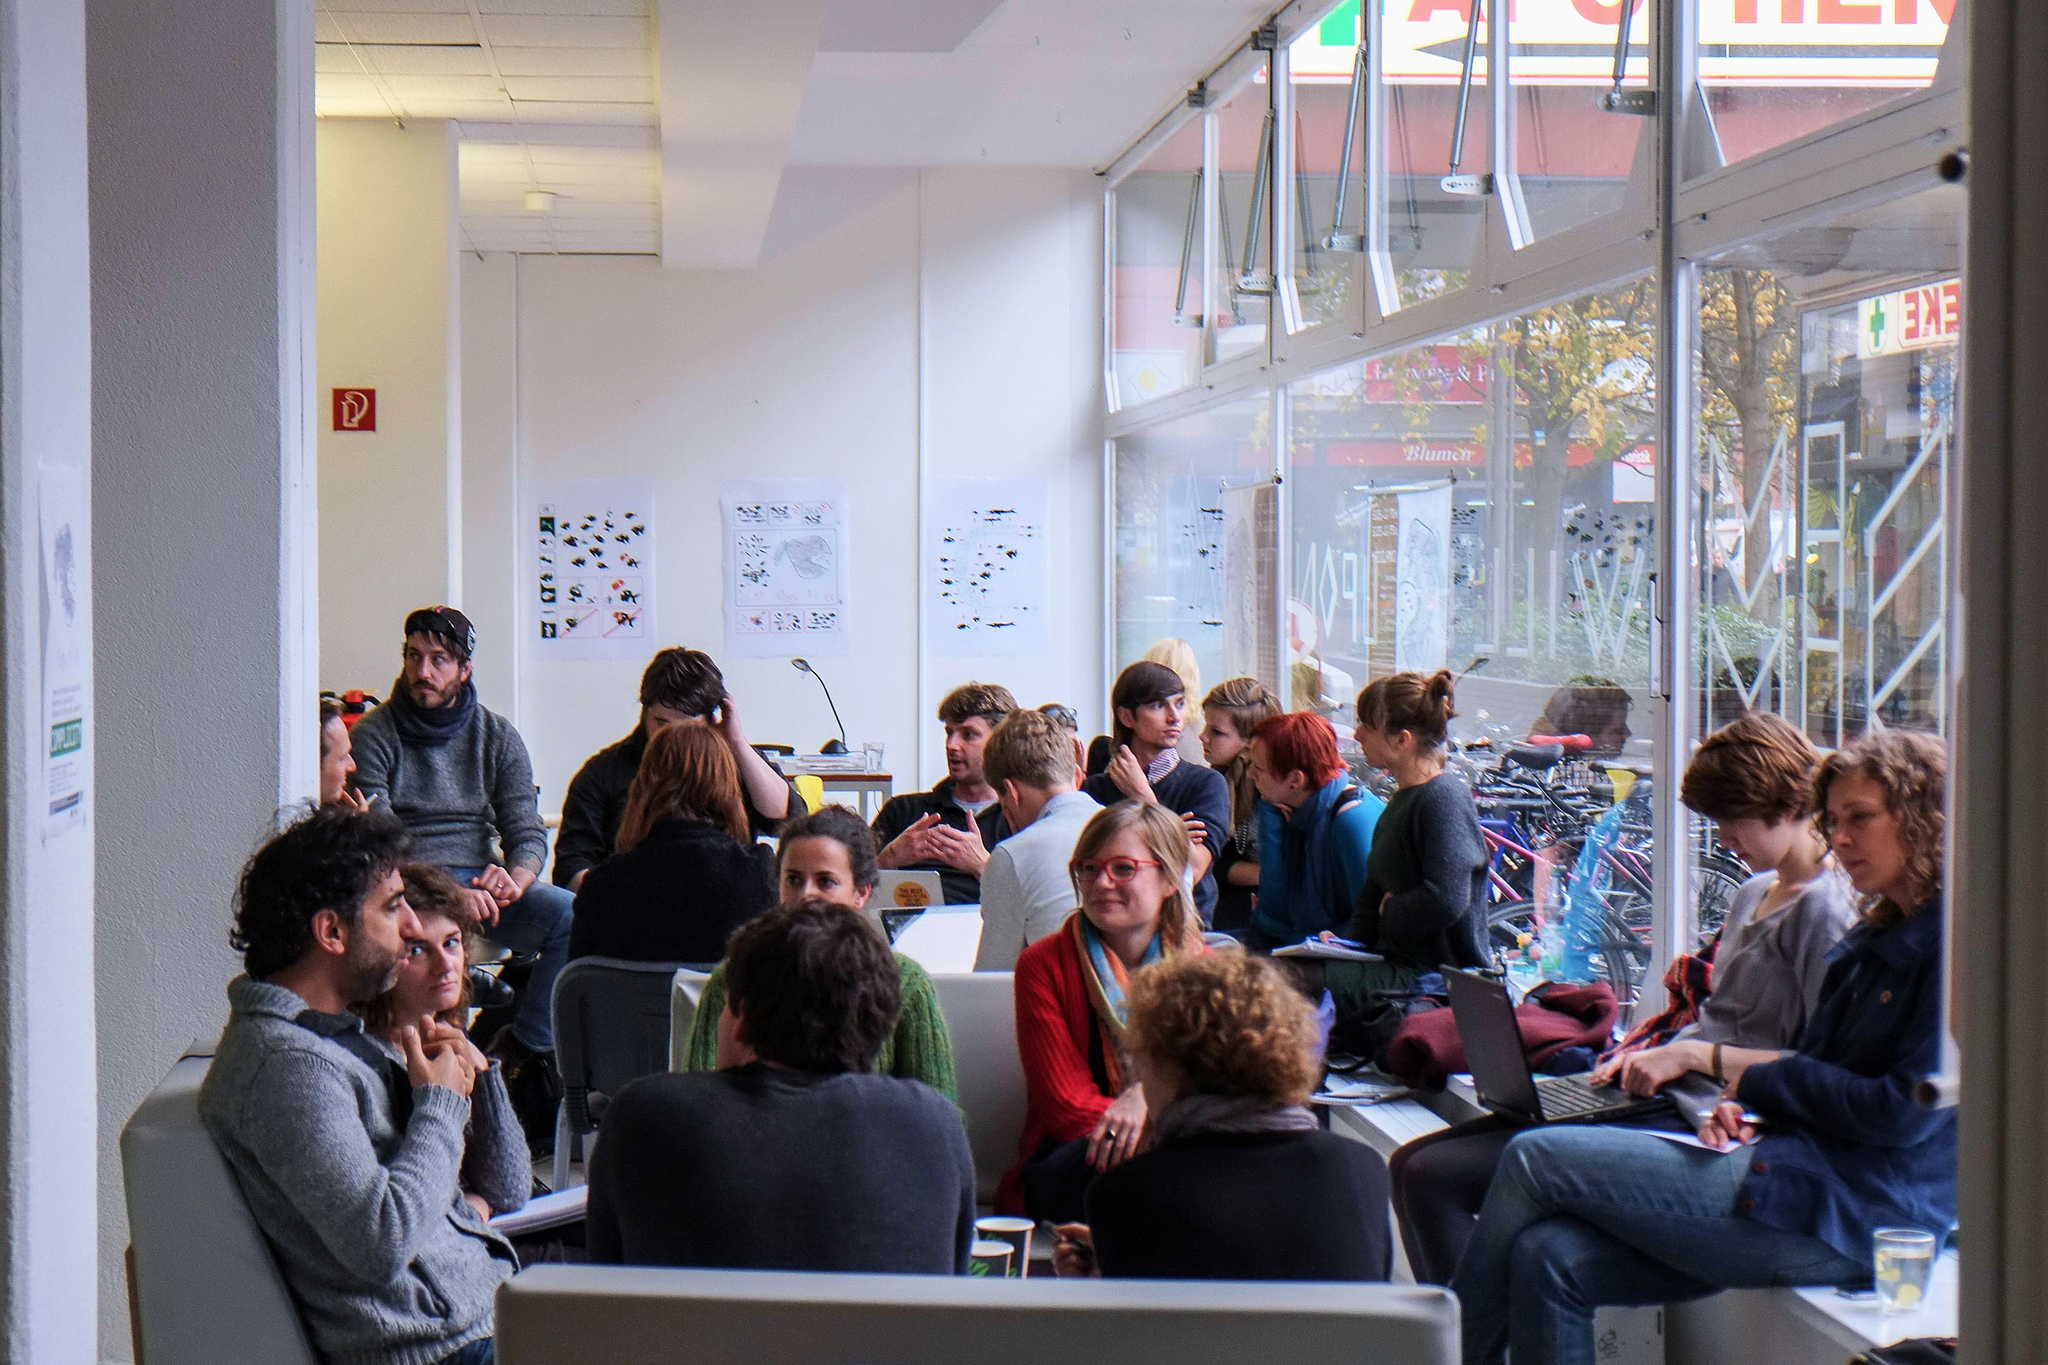
\includegraphics{./img/Konferenzteilnehmer.jpg}
\caption{Konferenzteilnehmer}
\end{figure}

\section*{Zwischen Traum und
Realität}\label{zwischen-traum-und-realituxe4t}

In dem Szenario der \enquote{Piraten und Kapitalisten} erscheint
\enquote{die Bibliothek} weniger als konkrete Institution denn als
Projektionsfläche für gesellschaftliche Utopien. Die Vision beschreibt
mit einer öffentlichen Universalbibliothek einen virtuellen Ort gelebten
Austausches, gelebter Demokratie von Gleichen. Wissen und Kultur gehören
der Gesellschaft und sind Gemeingut. Eine kommerzielle Ökonomie des
Wissens hat hier keinen Platz. Diese digitale Superbibliothek war schon
der Traum der Internetpioniere, bevor das Netz zum Shoppingparadies und
zur Zerstreuungshölle wurde, der datengetriebene Kapitalismus zum
Höhenflug ansetzte.

\section*{Kritische Fragen an die Utopie der globalen
Bibliothek}\label{kritische-fragen-an-die-utopie-der-globalen-bibliothek}

Doch nicht alle sind bereit, der Utopie zu folgen, ohne die immerhin
noch real existierende Bibliothekswelt unter die Lupe zu nehmen. Als wir
uns in kleine Untergruppen aufteilen, um einzelne Probleme zu
untersuchen, formiert sich ein gallisches Dorf (Iskra, Simon und
Corinna) zur Verteidigung der realen Bibliothek.

Die Kulturvermittlerin Iskra Geshoska aus Skopje, Simon Worthington, der
\enquote{Dreampunk} und Entwickler hybrider Leseformate aus
London/Lüneburg und die Bibliothekarin Corinna Haas aus Berlin denken
über \enquote{Libraries and Education} nach. \enquote{Was machen
Bibliotheken eigentlich?}, fragen Iskra und Simon die Autorin gleich zu
Beginn. Schnell zeigt sich, dass die beiden, und das dürfte für viele
andere Konferenzteilnehmer auch gelten, über die Aufgaben und aktuellen
Arbeitsschwerpunkte von Bibliotheken nicht sehr viel wissen: Die
zunehmende Anzahl von Digitalisierungsprojekten, die Entwicklung von
Standards für die digitale Langzeitverfügbarkeit, Aktivitäten im Bereich
Forschungsdatenmanagement, die Unterstützung von Forschungs- und
Publikationsprozessen, das Engagement von Bibliotheken im Gebiet
Leseförderung und Vermittlung von Informationskompetenz, die Rolle der
Bibliothek als gesellschaftlicher Raum und (physischer) Lernort und so
weiter. Auch wenn Anspruch und Wirklichkeit von Bibliotheken nicht immer
übereinstimmen, wird doch aus den Ausführungen der Bibliothekarin
schnell deutlich, dass Bibliotheken mehr leisten, als nur
Informationsressourcen bereit zu stellen, wie eine reine Datenbank --
sie unterstützen auf der Basis gemeinsamer gesellschaftlicher Werte
Lernen, Bildung und Forschung auf vielen Ebenen. (Und die Grenzen
zwischen Wissensinstitutionen wie Bibliothek, Schule und Universität
sind heute durchlässig geworden.)

Kritische Fragen, die unser gallisches Grüppchen dann unter der
Überschrift \enquote{The Library Protest} dem Plenum stellt, sind etwa:
Wollt Ihr wirklich Bibliotheken abschaffen oder für überflüssig
erklären? Wer sagt Euch, dass Ihr den Regierungen damit nicht nahe legt,
auch gleich die Universitäten zu schließen und durch Online-Vorlesungen
zu ersetzen? Und danach die Schulen?

Die Großgruppe der Piraten reagiert ein wenig irritiert auf unsere
Präsentation, da wir uns nicht auf die Island-Utopie eingelassen hätten.
Vielleicht, um uns wieder ins Boot zu holen, interpretiert dann jemand
unsere reale Bibliothek als \enquote{universal classroom} -- und führt
sie so in die utopische Sphäre zurück.

\begin{figure}[htbp]
\centering
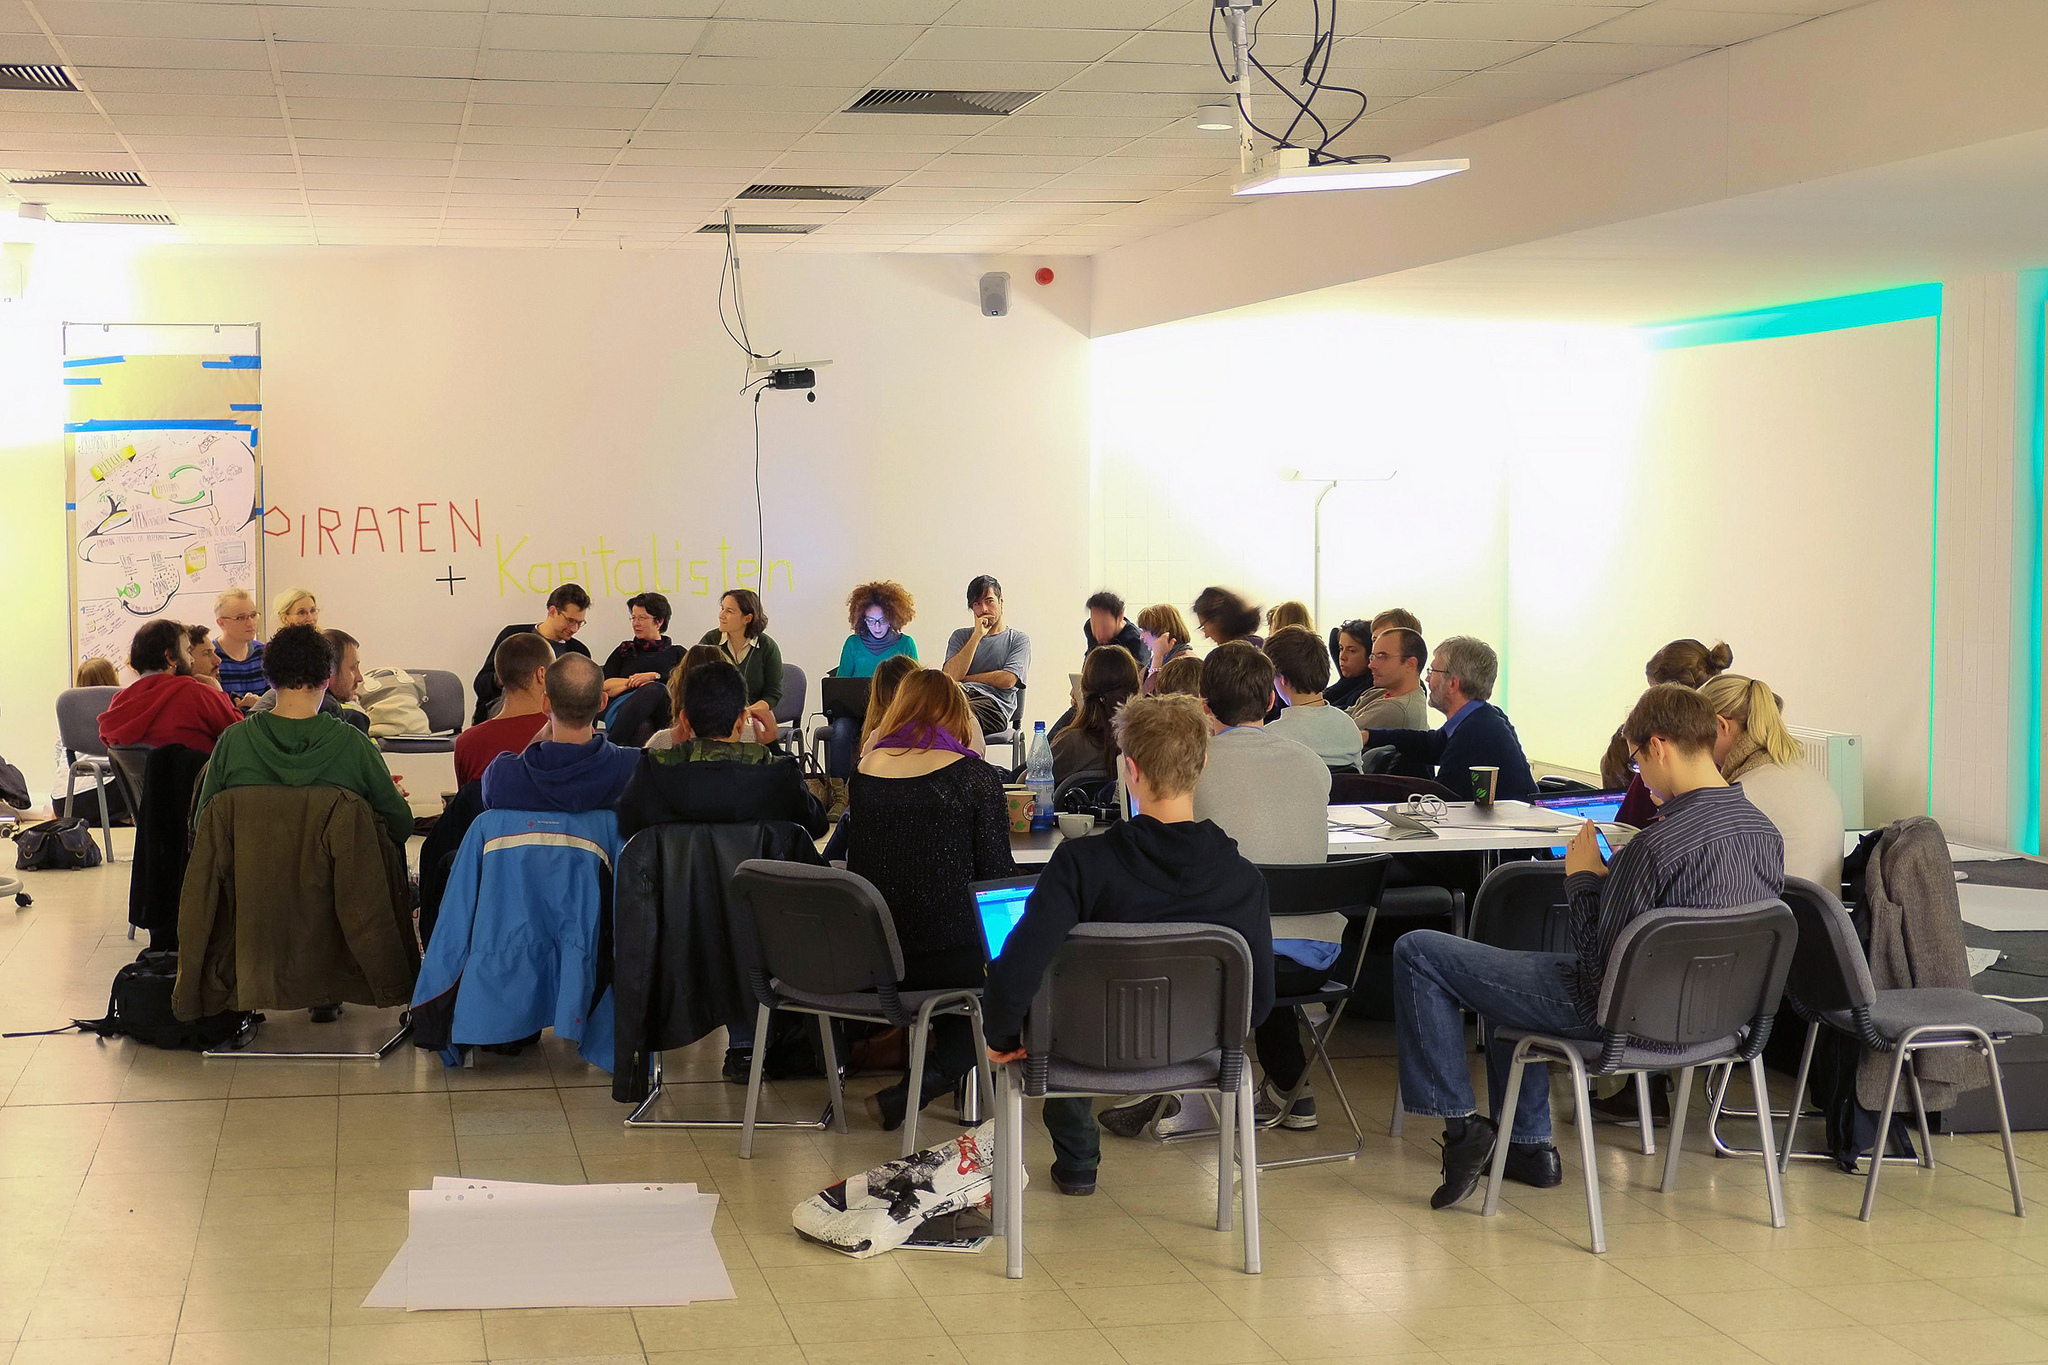
\includegraphics{./img/WorkshopPiratenundKapitalisten.jpg}
\caption{Workshop Piraten und Kapitalisten}
\end{figure}

\section*{Vertraute Thesen}\label{vertraute-thesen}

Die Utopisten vertreten derweil vertraute Thesen, stellen Fragen, wie
wir Bibliothekarinnen sie aus der frühen Open Access-Bewegung kennen:
Wozu braucht es Verlage, wenn wir doch alle selber Verleger sein können?
Spielen die Verwertungsgesellschaften nicht eher eine unheilige Rolle?
Sind Initiativen wie die Cultural Commons Collecting Society, kurz
C3S,\footnote{\url{https://www.c3s.cc/}} als Gegenmodell zur Gema ein
Vorbild auch für Wortkünstler? Ist das mit dem Urheberrecht verbundene
Geldversprechen für Künstler wirklich mehr als ein großes Glücksspiel?
Werden hier nicht vor allem die Zwischenhändler, Agenturen, Verlage
geschützt? Die Forderung:\enquote{Cut the middleman!} wird auf
\emph{Graphic Recordings} festgehalten. Am Ende der Diskussion steht auf
einem Plakat der Ausspruch: Nicht jeder Künstler kann Lady Gaga sein.
Nicht jeder wird mit seinem Werk Millionen verdienen können.
Urheberrecht hin, Urheberrecht her.

\section*{Lessons Learned}\label{lessons-learned}

Wir haben bei der Complicity-Konferenz sehr viel von Journalisten,
Kreativen und Programmierern über ihre Probleme mit und ihre Sicht auf
das geltende Urheberrecht gelernt. Wir waren beeindruckt von der Energie
und dem \emph{community spirit} unter den Konferenzteilnehmern. Und wir
haben uns erzählen lassen, was von Bibliotheken -- utopischen und realen
-- erwartet wird:

\textbf{1. Die Zukunft der Bibliotheken findet sich in ihrer
Vergangenheit.} Wenn Bibliotheken sich auf ihre Grundaufgabe, Zugänge zu
Information und Bildung zu schaffen, zurück besinnen, haben sie auch im
digitalen Zeitalter eine Jahrhundertaufgabe vor sich.

\textbf{2. Je ungelöster die Urheberrechtsprobleme, desto attraktiver
wird piratisches Handeln}. Wer hat noch nie einen Musiktitel geteilt
oder eine PDF-Datei weiter geschickt? Die Behinderung wissenschaftlicher
Arbeit durch rechtliche und finanzielle Hürden wird längst nicht mehr
widerstandslos hingenommen. Seht hin, Bibliothekare: Wissenschaftler
versorgen sich mit Literatur aus illegalen Datenbanken und packen am
Rande von Konferenzen ihre Festplatten aus, um \enquote{befreite Bücher}
auszutauschen. Und \enquote{Piraten} arbeiten fleißig daran, immer
größere illegale Datenbanken aufzubauen.

\textbf{3. Je sozial akzeptierter piratisches Handeln, desto größer wird
der Druck der \enquote{kritischen Masse} auf den Gesetzgeber.} Die
Gesetzgebung ist träge und hinkt zwangsläufig gesellschaftlichen und
technologischen Entwicklungen regelmäßig hinterher. Doch wie viele
illegale Downloads und illegale Digitalisierungen muss es noch geben,
damit das Urheberrecht für die Wissenschaften und die lernende
Gesellschaft eine zeitgemäße und praktikable Form erhält? Denn selbst
wenn man es wollte, könnte man nach den bestehenden Vorgaben kaum beides
haben: Absolut urheberrechtskonform handeln und zugleich an der
digitalen Kultur und der digitalen Wissenschaft teilhaben.

\textbf{4. Internetaktivisten und Bibliothekare wissen viel zu wenig
voneinander!} Vielleicht liegt es am unterschiedlichen professionellen
Habitus und der großen Kluft, die Bibliothekare vom
\enquote{intelligenten Leben jenseits der Festanstellung} (Friebe/Lobo
2006) trennt: Jedenfalls wissen Bibliothekare und Internetaktivisten
offenbar sehr wenig voneinander. Dabei gleichen sich ihre Ziele auf
verblüffende Weise: Beide Gruppen wollen den freien Zugang zur
Information! Eine größere Offenheit auf beiden Seiten und sehr viel mehr
\enquote{fachfremder} Austausch wären dienlich. Es gibt dafür
Veranstaltungsformate - die Berliner Gazette hat es vorgemacht. Machen
wir es nach!

\section*{Komplizen}\label{komplizen}

Das theoretische Konzept zu der Veranstaltung \enquote{Complicity --
Komplizenschaft} lieferte die Hamburger Philosophin und
Kulturanthropologin Geza Ziemer (Ziemer 2013) am letzten Tag. Mit dem
Konzept der \enquote{complicity} beschreibt sie Formen der Konnektivität
und der Kollaboration, die sich in den letzten Jahren entwickelt haben.
Sie definiert Komplizenschaft als lose Verbindung zwischen Menschen, die
sich in der Regel jenseits der Gesetze zu einer Tat verabreden. Es sind
zufällige Begegnungen, die Menschen zu Komplizen machen. Komplizen
suchen sich nicht, sie finden sich und das oftmals nonverbal (etwa durch
mimische Signale). Komplizen verständigen sich, planen, handeln und
gehen danach wieder auseinander. Das unterscheidet Komplizenschaften von
Netzwerken (in denen man passiv bleiben kann) oder festen kollegialen
Strukturen.

\begin{figure}[htbp]
\centering
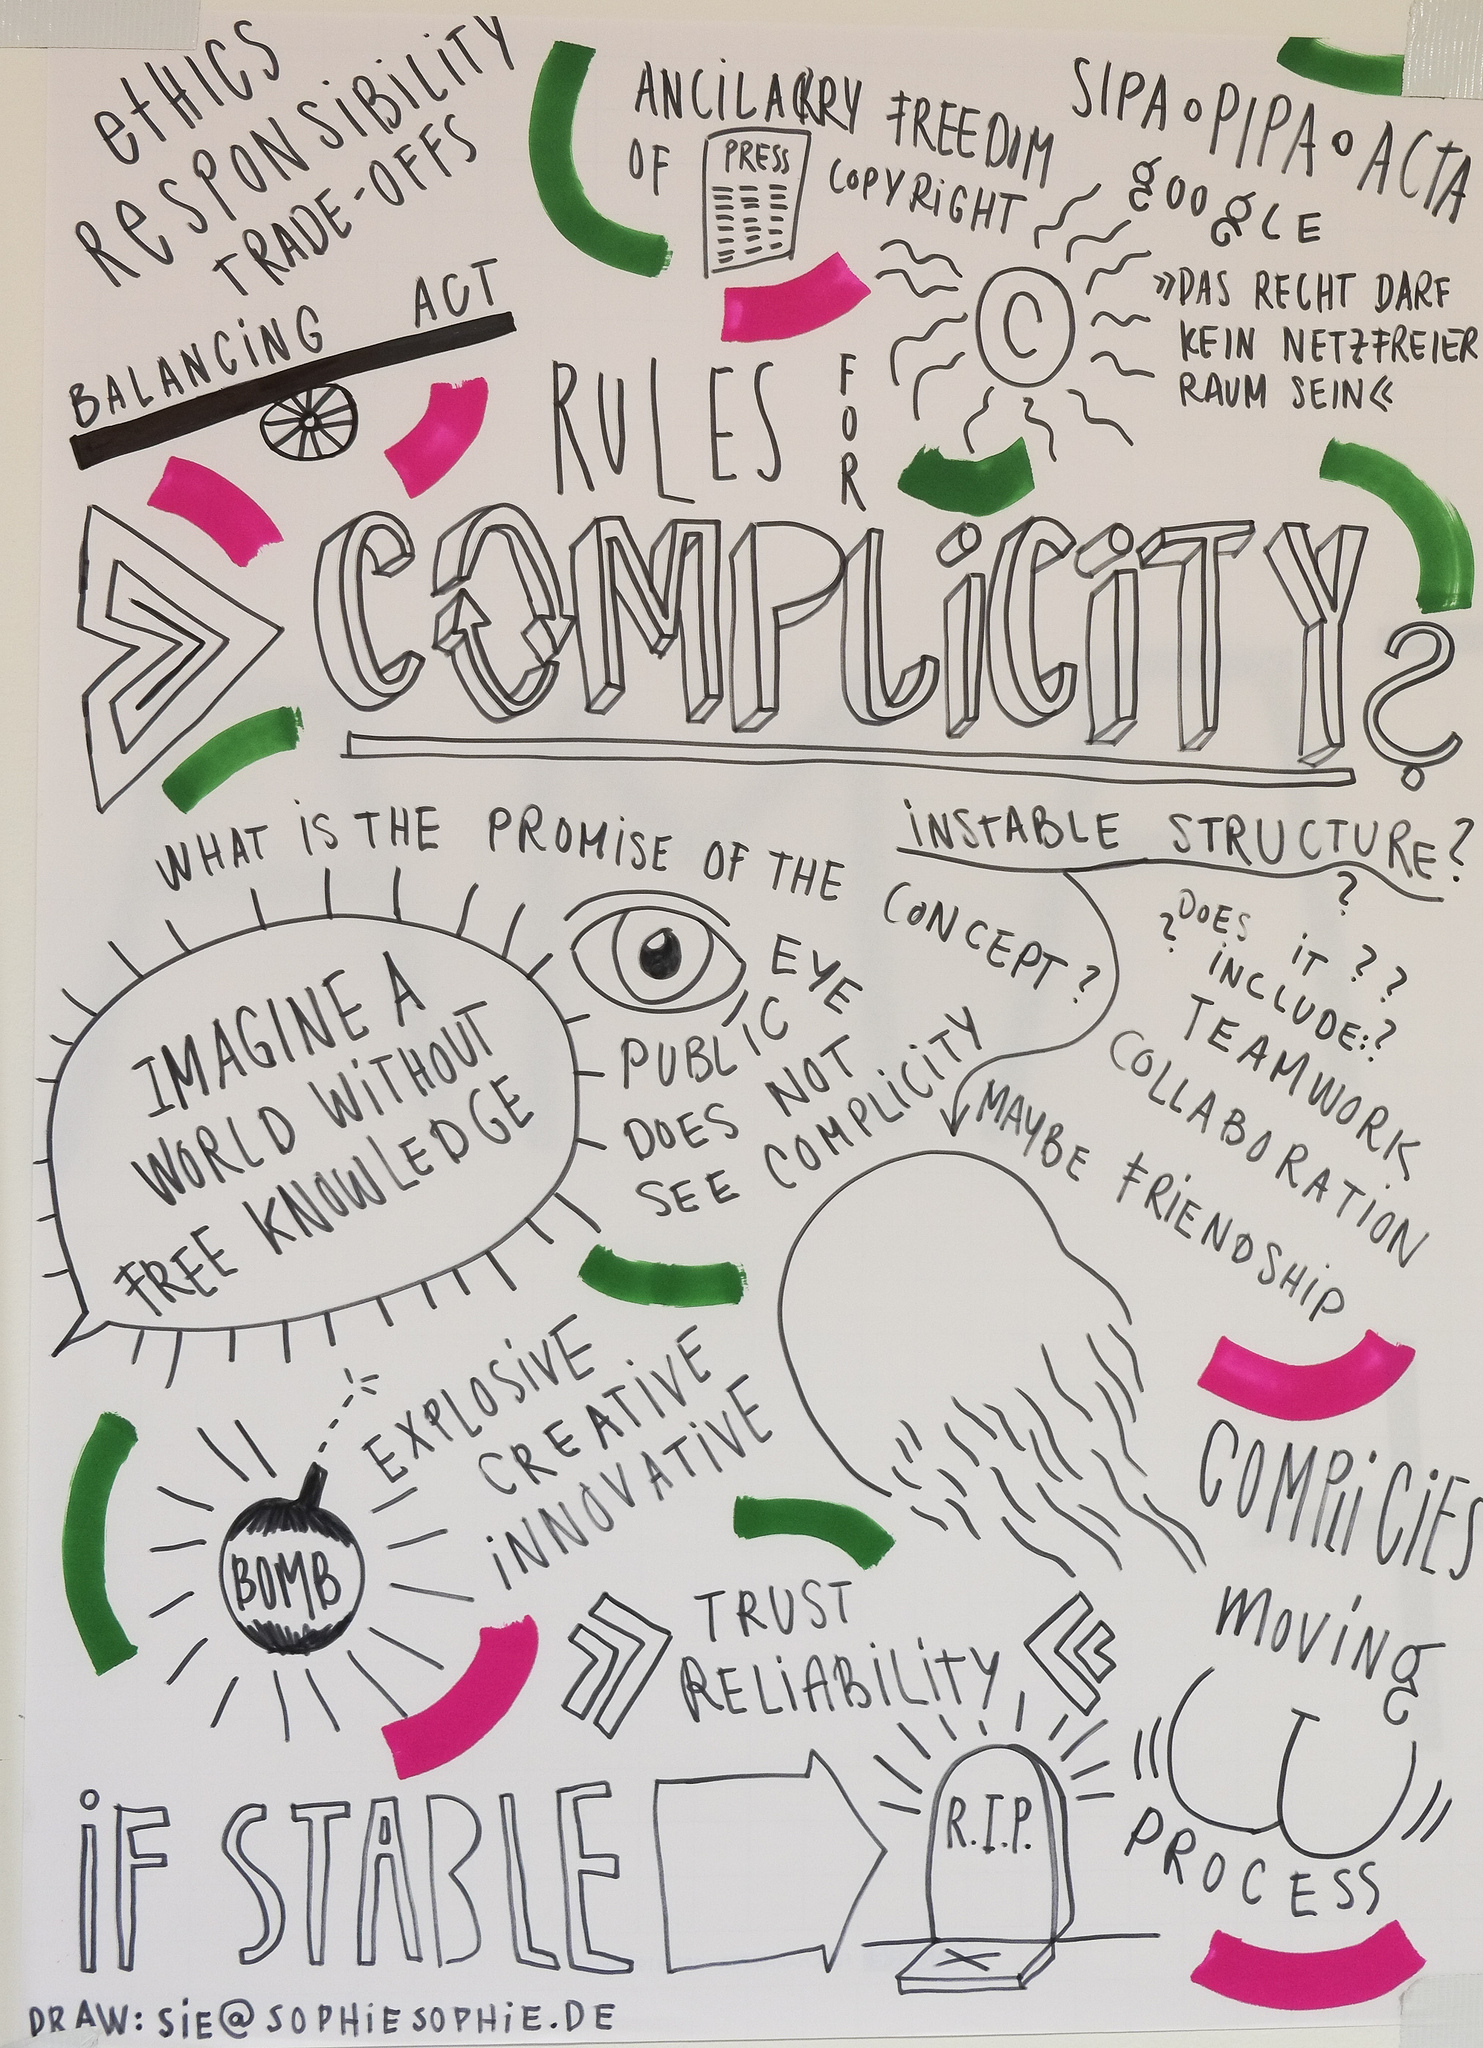
\includegraphics{./img/GraphicRecording_02.jpg}
\caption{Graphic Recording}
\end{figure}

Weitere Vorträge stellen gelebte -- oder auch konstruierte, denkbare --
Komplizenschaften vor. Da berichten unter der Überschrift
\enquote{Hacker und Journalisten} Sebastian Candea, Journalist aus
Bukarest und Stefan Mondial, Programmierer aus Deutschland, über das
investigative Projekt Offshore Leaks.\footnote{\url{http://www.icij.org/offshore}}
Beispiele einer gelungenen Zusammenarbeit von \enquote{Amateuren und
Profis} im Bereich~ Musik benennen Mitsuhiro Takemura, Crypton Future
Media und Valje Djordjevic, iRights Media Berlin. Eindrucksvoll
vermessen sie die Überschneidungen zwischen kommerzieller
Musikproduktion, Fankultur und Nutzerkreativität. Zitiert wird dies am
Beispiel der Gesangssoftware Hatsune Miku, die sich in Asien zu einem
populären Trend entwickelt hat und nun auch Europa erreicht hat. Eine
glückliche Verbindung von \enquote{Kapitalisten und Piraten} findet
Michiel de Jong schließlich im Projekt Opentabs, das dazu beitragen
soll, ein Wirtschaftssystem ohne Banken zu etablieren.\footnote{\url{http://opentabs.net/}}

Internet- und Medienaktivisten, CopyLeft-Advokaten -- die Komplizen der
Bibliotheken wissen sehr, sehr gut Bescheid. Sie kennen die Nöte der
Bibliotheken, die Tücken des Urheberrechts, die Fallstricke in den
Lizenzverträgen mit Wissenschaftsverlagen, die Grenzen der Onleihe und
die Hürden auf dem Weg zu einer freien, digitalen Privatkopie. Je
radikaler die Komplizen, desto weniger wollen sie die Bibliothek als
besseren Coworking Space. Stattdessen sollen die Bibliotheken sich auf
ihre alten Werte, die Demokratisierung des Wissens, Zugänglichkeit zu
schaffen, auch im digitalen Zeitalter rückbesinnen. Die Öffentliche
Bibliothek als Idee hat nicht ausgedient, im Gegenteil gilt es für diese
Idee neu zu kämpfen. Das wurde besonders deutlich in Gesprächen mit
Intellektuellen aus Ländern, in denen weder politisch noch ökonomisch
die Voraussetzungen für den freien Zugang zu Informationen und Bildung
und die entsprechenden Institutionen, also Bibliotheken, gegeben sind.

Manche unserer Komplizen fangen schon einmal an und füllen illegale
Portale wie Library Genesis,\footnote{\url{http://lib.freescienceengineering.org/view.php?id=549037}}
oder sie engagieren sich in Kunstprojekten wie
memoryoftheworld.org.\footnote{Marcell Mars stellt memoryoftheworld z.
  B. in diesem Podcast vor: \url{http://vimeo.com/60889534}} Aber auch
unsere gar nicht so fernen Nachbarn in Norwegen machen Nägel mit Köpfen:
Die norwegische Nationalbibliothek erklärte im Dezember 2013, den
Gesamtbestand norwegischer Literatur digitalisieren und für den
norwegischen IP-Bereich frei zugänglich machen zu wollen. Allerdings
steht nur Literatur mit Erscheinungsjahr bis 2001 für Leser kostenfrei
online zur Verfügung. Dem vorausgegangen war eine Einigung der
norwegischen Rechteinhabern und der Bibliothek.\footnote{Mehr
  Informationen zur norwegischen Digitalisierungsinitiative:
  \url{http://www.lesen.net/ebook-news/der-staat-zahlt-norweger-koennen-kommerzielle-ebooks-kostenlos-online-lesen-9430}}
Mit dieser Initiative rückt das auf der Konferenz leidenschaftlich
beschworene Szenario in einem Teil von Europa schon ein wenig näher. So
bleibt am Ende die Frage: Mit welchen Komplizen können sich
Bibliothekare verbünden, damit die deutsche Bibliothekslandschaft
\enquote{norwegischer} wird?

\section*{Literatur}\label{literatur}

Friebe, Holm ; Lobo, Sascha (2006): Wir nennen es Arbeit. Die digitale
Bohème, oder: Intelligentes Leben jenseits der Festanstellung, München:
Heyne

Taube, Magdalena ; Woznicki, Krystian (2014, erscheint demnächst):
Komplizen. Wie können Hacker und Journalisten, Piraten und Kapitalisten,
Amateure und Profis zusammenarbeiten? Berlin, iRights Media (Ebook)

Ziemer, Gesa (2013): Komplizenschaft. Neue Perspektiven auf
Kollektivität Bielefeld: Transcript

\end{document}